% !TeX spellcheck = cs_CZ
%{\tikzset{external/prefix={tikz/FYZII/}}
% \tikzset{external/figure name/.add={ch19_}{}}
%---------------------------------------------------------------------------------------------------
% file fey2ch19.tex
%---------------------------------------------------------------------------------------------------
%=========================== Kapitola Princip nejmenší akce ========================================
\setchaptertoc
\chapter{Princip nejmenší akce}\label{fyz:IIchapXIX}

  \luagraphic[1]{fyz_fig650.jpg}{Speciální přednáška - s Feynmanovými náčrtky na tabuly
  (\cite[s.~707]{Feynman02})}{fyz:fig650}

  \section{Speciální přednáška - s Feynmanovými náčrtky na tabuly}\label{fyz:IIchapXIXsecI}
    Můj učitel fyziky mi řekl toto: „Dejme tomu, že máš nějakou částici třeba v gravitačním poli,
    která se začne odněkud pohybovat a volně se blíží k nějakému jinému bodu. Můžeš ji třeba hodit,
    takže bude stoupat a potom zase klesat. Bude se pohybovat z původního místa ke konečnému místu a
    tento pohyb trvá určitou dobu. Nyní si mysli nějaký jiný pohyb. Nechť se částice na své dráze
    pohybuje tak, jak je znázorněno na druhém obrázku vpravo, ale doba trvání pohybu je stejná jako
    v prvním případě.“ A pak můj učitel dodal: „Vypočítáš-li jakou má částice v každém okamžiku na
    své dráze kinetickou energii, odečteš-li od ní potenciální energii a integruješ podle času přes
    časový interval potřebný k průchodu celé dráhy, dostaneš číslo, které je větší než číslo
    odpovídající skutečnému pohybu.

    \begin{figure}[ht!]  
      \centering
      \begin{tabular}{cc}
        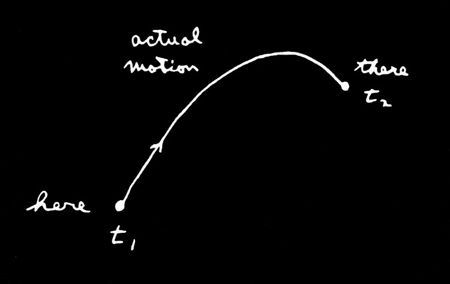
\includegraphics[width=0.450\linewidth]{fyz_fig651.jpg}              &                                                       
        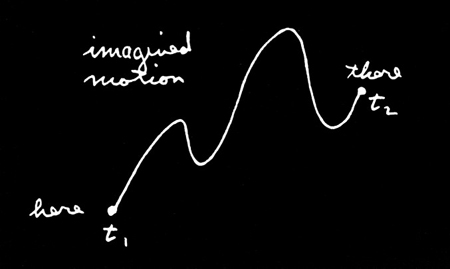
\includegraphics[width=0.465\linewidth]{fyz_fig652.jpg}
      \end{tabular}
    \end{figure}

    Jinak řečeno: Newtonovy zákony mohou být formulovány ne ve tvaru \(F=ma\), ale ve tvaru, který
    odráží skutečnost, že střední kinetická energie minus střední potenciální energie má nejmenší
    hodnotu na té dráze, po které se předmět ve skutečnosti pohybuje od jednoho místa k druhému.“

    Vysvětlíme si blíže, co to vlastně znamená. Budeme-li se zajímat o pohyb v gravitačním poli, pak
    při pohybu částice po dráze \(x(t)\) (nejdříve budeme uvažovat jednorozměrný problém a budeme
    předpokládat, že částice se pohybuje jen nahoru a dolů, a ne do strany), kde \(x\) je výška nad
    zemí, bude kinetická energie rovna \(1/2 m(\frac{dx}{dt})^2\) a potenciální energie bude v
    každém okamžiku rovna \(mgx\). Nyní vezměme rozdíl kinetické a potenciální energie v každém
    okamžiku pohybu a tento výraz integrujeme podle času od počátečního do konečného okamžiku.
    Předpokládejme, že v počátečním čase \(t_1\), tento pohyb začínal v určité výšce a v konečném
    čase \(t_2\), pohyb skončil v nějakém jiném místě. 

    Pak máme integrál
    \begin{equation*}
      \bigint_{t_1}^{t_2}\left[\frac{1}{2}m\left(\der{x}{t}\right)^2 - mgx\right]\dd{t}
    \end{equation*}

    Skutečný pohyb se děje po určité křivce (vyjadřujeme-li závislost na čase, jde o parabolu) a pro
    ni dostáváme určitou hodnotu uvedeného integrálu. Můžeme si však představit nějaký jiný pohyb,
    kdy by se částice pohybovala nahoru a dolů nějakým neobvyklým způsobem.
    
    \begin{figure}[ht!]  
      \centering
      \begin{tabular}{cc}
        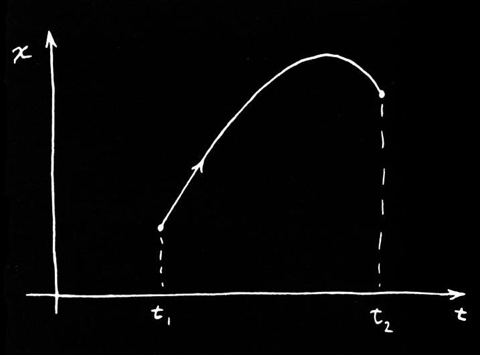
\includegraphics[width=0.47\linewidth]{fyz_fig653.jpg}             &                                                        
        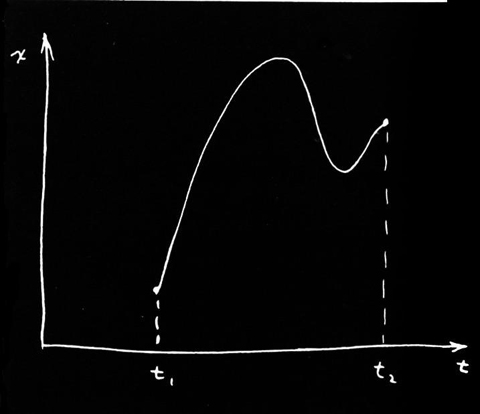
\includegraphics[width=0.41\linewidth]{fyz_fig654.jpg}
      \end{tabular}
    \end{figure}

    Pro takový pohyb pak můžeme vypočítat rozdíl kinetické a potenciální energie a tento rozdíl
    integrovat po znázorněné křivce... nebo po jakékoliv jiné křivce. Podstatné je, že tou pravou
    křivkou je ta, pro níž má tento integrál \textbf{nejmenší hodnotu}.

    Vyzkoušejme to. Nejdříve si všimněme pohybu volné částice, která nemá žádnou potenciální
    energii. Pravidlo pak říká, že při pohybu z jednoho místa na druhé v dané době musí být integrál
    kinetické energie nejmenší, takže pohyb se musí dít konstantní rychlostí. (My už víme, že
    správnou odpovědí je pohyb konstantní rychlostí.) Proč je tomu tak? Proto, že při jiném pohybu
    částice by byly rychlosti někdy větší a někdy menší než průměr. Jenže průměrná rychlost je vždy
    stejná, neboť všechny pohyby z jednoho místa na druhé se uskutečňují ve stejném čase.

    Jako příklad nám poslouží situace, kdy máme jet z domova do školy autem a cesta nám má trvat
    určitou dobu. Cestu můžeme uskutečnit různými způsoby. Na začátku můžeme divoce zrychlovat a
    před koncem silně brzdit, nebo můžeme jet konstantní rychlostí, nebo můžeme jet chvíli zpátečkou
    a potom opět dopředu, nebo si můžeme zvolit ještě jiné způsoby. Je důležité, že průměrná
    rychlost je podíl projeté vzdálenosti a času potřebného na cestu. Kromě případu konstantní
    rychlosti pojedeme vždy tak, že někdy pojedeme příliš rychle a někdy pojedeme příliš pomalu. Ale
    střední hodnota druhých mocnin hodnot, které se liší od průměru, je, jak víme vždy větší než
    druhá mocnina střední hodnoty, a proto bude integrál kinetické energie vždy větší při kolísání
    rychlosti než při rychlosti konstantní. Vidíme tedy, že integrál má minimum, je-li rychlost
    konstantní (když není žádné silové působení). Správná křivka vypadá jako na obrázku vlevo.
    
    \begin{figure}[ht!]  
      \centering
      \begin{tabular}{cc}
        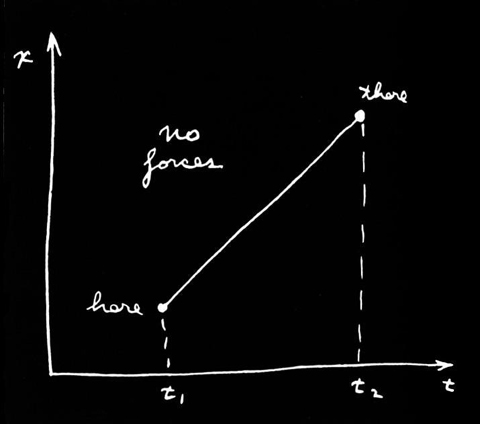
\includegraphics[width=0.455\linewidth]{fyz_fig655.jpg}             &                                                        
        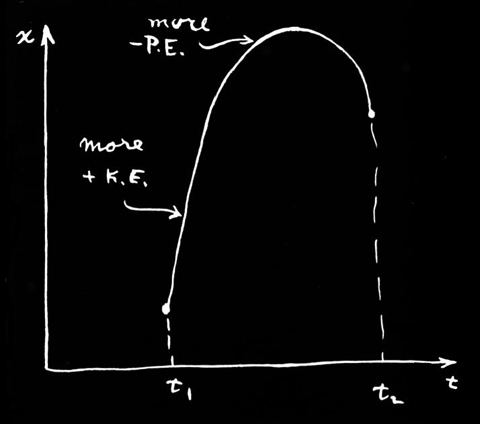
\includegraphics[width=0.440\linewidth]{fyz_fig656.jpg}
      \end{tabular}
    \end{figure}

    Předmět vržený vzhůru v gravitačním poli se pohybuje nejdříve rychle, ale potom stále pomaleji.
    Je to proto, že má i potenciální energii a nejmenší musí být rozdíl kinetické a potenciální
    energie. Protože potenciální energie roste s výškou, bude rozdíl co nejmenší, když se co
    nejrychleji dostaneme nahoru, kde je velká potenciální energie. Potom odečteme-li potenciální
    energii od kinetické, dostaneme menší střední hodnotu. Výhodnější je taková křivka, která rychle
    stoupá a při níž se odečítá mnoho potenciální energie.

    Nemůžeme však stoupat příliš rychle nebo příliš vysoko, neboť pak by byla velká i kinetická
    energie. Přitom je třeba stoupat dost rychle, aby bylo možné vrátit se v určeném čase. Nechceme
    tedy příliš vysoko, ale kamsi přece jen vystoupit chceme. Řešením je tedy určitá rovnováha mezi
    snahou o získání co největší potenciální energie při co nejmenším nárůstu kinetické energie. Jde
    o to, aby rozdíl kinetické a potenciální energie byl co nejmenší.

    Matematický problém, který budeme řešit, je obtížný a nezvyklý. Budeme se zabývat určitou
    veličinou nazývanou \text{akce (účinek)} \(S\). Je to rozdíl kinetické a potenciální energie
    integrovaný podle času.
    \begin{equation*}
      \text{akce} = S = \int_{t_1}^{t_2}\left(KE - PE\right)\dd{t}
    \end{equation*}

    Musíme si uvědomit, že \(PE\) a \(KE\) jsou funkce. Pro různé možné křivky bude akce nabývat
    různých hodnot. Naší matematickou úlohou je najít, pro kterou křivku je toto číslo nejmenší.

    Možná že si řekneme: „Je to obyčejný výpočet maxima a minima. Je třeba vypočítat akci a
    derivováním najít minimum.“

    Ale pozor! Obvykle máme funkci nějaké proměnné a hledáme hodnotu proměnné, při které je funkce
    menší nebo větší. Můžeme mít například tyč, která byla zahřáta uprostřed a odtud se teplo šíří
    dále. Každý bod tyče bude mít určitou teplotu a máme najít bod, v němž je teplota největší. My
    však máme pro každou křivku v prostoru určité číslo (tedy něco docela jiného) a hledáme takovou
    křivku, pro níž je toto číslo nejmenší. Taková úloha patří do docela jiné oblasti matematiky. To
    už není obyčejný integrální a diferenciální počet. Podobné výpočty patří do variačního počtu.

    Problémů tohoto typuje v matematice mnoho. Například kružnice je obvykle definována jako
    geometrické místo bodů v rovině, které jsou stejně vzdáleny od nějakého bodu. Existuje však
    i jiná definice kružnice. Kružnice je taková křivka dané délky, která obepíná největší plochu.
    Každá jiná uzavřená křivka se stejným obvodem obepíná menší plochu než kružnice. Stanovíme-li
    tedy problém najít křivku, která při daném obvodu obepíná největší plochu, dostaneme úlohu
    variačního počtu, což je něco docela jiného než úlohy, na které jsme byli
    zvyklí.

    \begin{figure}[ht!]  
      \centering
      \begin{tabular}{cc}
        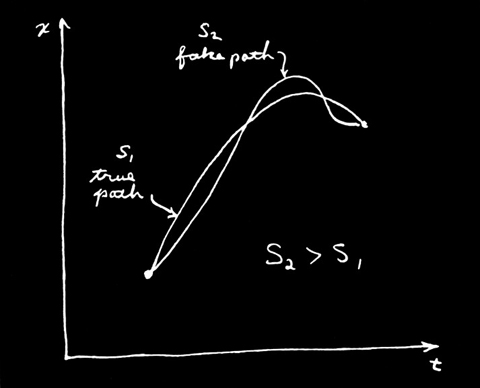
\includegraphics[width=0.400\linewidth]{fyz_fig657.jpg}             &                                                        
        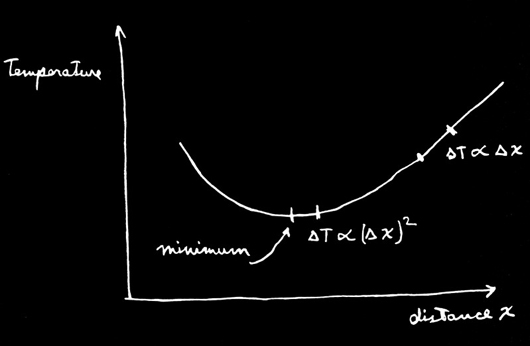
\includegraphics[width=0.490\linewidth]{fyz_fig658.jpg}
      \end{tabular}
    \end{figure}
    
    Budeme tedy počítat křivku, podle níž se těleso bude pohybovat. Uděláme to následujícím
    způsobem. Představíme si, že existuje ta pravá křivka a všechny ostatní křivky jsou nepravé.
    Budeme-li počítat akci pro nepravou křivku, dostaneme větší hodnotu než při výpočtu akce pro
    pravou křivku.
    
    Naší úlohou je najít pravou křivku. Kde taková křivka leží? Jeden ze způsobů určení spočívá v
    tom, že budeme počítat akci pro milióny a milióny křivek a budeme zkoumat, pro kterou křivku je
    akce nejmenší. Když to zjistíme, najdeme tu pravou křivku.

    Tak bychom mohli opravdu postupovat. Můžeme to však udělat o něco lépe. Jde-li o obyčejnou
    funkci, která má minimum (např. o teplotu), můžeme využít té vlastnosti minima, že při
    vzdalování od minima na vzdálenost \emph{prvního} řádu, se změní hodnota funkce pouze o
    veličinu, která je \emph{druhého} řádu. V jakémkoliv jiném bodě křivky se při malé změně
    proměnné změní hodnota funkce o veličinu, která je i prvního řádu. Ale v minimu nezpůsobuje
    posun o malou vzdálenost v prvním přiblížení žádné změny funkce.

    Toho využijeme při výpočtu naší křivky. Je-li křivka pravá, nebude mít křivka, která se od ní
    pouze nepatrně liší, v prvním přiblížení jinou akční funkci. Jde-li opravdu o minimum, objeví se
    rozdíly až ve druhém přiblížení.
    
    Lze to snadno dokázat. Změníme-li nějakým způsobem křivku tak, aby změna byla prvního řádu,
    změní se úměrně tomu i akce. Při této změně se akce stává podle předpokladu větší, neboť jinak
    by nešlo o minimum. Je-li však změna úměrná odchylce, při změně znaménka by se vlastně akce
    zmenšovala. Dostali bychom situaci, kdy akce roste při odchýlení na jednu stranu a klesá při
    odchýlení na stranu opačnou. Je jen jedna možnost, abychom dostali minimum, a to ta, že v prvním
    přiblížení nedochází ke změnám a změny jsou úměrné druhé mocnině odchylky od pravé křivky.
    Budeme proto postupovat takto. Symbolem \(\underline{x(t)}\) (s čarou dole) označíme pravou
    křivku, tu, kterou se snažíme najít. Vezmeme nějakou zkušební křivku \(x(t)\), která se od té
    pravé liší o malou hodnotu, a tu označíme \(\eta(t)\).

    \luagraphic[1]{fyz_fig659.jpg}{Tabule s náčrty (\cite[s.~336]{Feynman02})}{fyz:fig659}

    Základní myšlenka spočívá v tom, že rozdíl mezi akcí \(\underline{S}\) podél křivky
    \(\underline{x(t)}\) a akcí \(S\) podél pravé křivky \(x(t)\) musí být v prvním přiblížení
    malého \(\eta(t)\) nulový. Tyto veličiny se mohou lišit ve druhém řádu, ale v prvním řádu musí
    jejich rozdíl být nulový.

    A přitom musí platit pro všechna \(\eta\). Ačkoliv to není docela pravda, neboť metoda ztrácí
    smysl pro jiné křivky než ty, které začínají a končí v týchž bodech. Každá křivka začíná v
    určitém bodě v čase \(t_1\), a končí v jiném bodě v čase \(t_2\), přičemž tyto body a časy jsou
    pevně dány. Naše funkce \(\eta\) tedy musí být nulová na obou koncích, takže \(\eta(t_1)=0\) a
    \(\eta(t_2)=0\). Touto podmínkou je náš matematický problém už úplně určen.

    Kdybychom neznali diferenciální počet, mohli bychom uvedený způsob použít k určení minima
    obyčejné funkce \(f(x)\). Mohli bychom uvážit, co se stane, vezmeme-li \(f(x)\) a přidáte malou
    veličinu \(h\) k \(x\), a mohli bychom dokázat, že korekce k \(f(x)\) podle \(h\) musí být v
    prvním řádu nulová. Místo \(x\) bychom dosadili \(x+h\) a rozvinuli do prvního řádu v
    \(h\ldots\) právě tak, jak se to chystáme udělat pro \(\eta\).

    Podstata našeho postupu bude spočívat v tom, že do výrazu pro akci
    \begin{equation*}
      S = \bigint\left[\frac{m}{2}\left(\der{x}{t}\right)^2 - V(x) \right]\dd{t}
    \end{equation*}
    v němž \(V(x)\) představuje \emph{potenciální energii}, zavedeme substituci \(x(t) =
    \underline{x(t)}+\eta(t)\). Derivace \(dx/dt\) je, samozřejmě, derivace \(\underline{x(t)}\)
    plus derivace \(\eta(t)\), takže pro akci dostaneme vyjádření
    \begin{equation*}
      S = \bigint\left[\frac{m}{2}\left(\der{\underline{x}}{t}+\der{\eta}{t}\right)^2 
          - V(\underline{x}+\eta)\right]\dd{t}
    \end{equation*}
    Nyní tento výraz rozepíšeme podrobněji. Pro člen s druhou mocninou dostaneme
    \begin{equation*}
      \left(\der{\underline{x}}{t}\right)^2 + 2\der{\underline{x}}{t}\der{\eta}{t} 
      + \left(\der{\eta}{t}\right)^2.
    \end{equation*}
    Ale pozor! Nás nezajímají členy, které jsou vyššího řádu než prvního, a proto členy obsahující
    \(\eta^2\) a vyšší mocniny zasuneme do škatulky zvané „druhý řád a řády vyšší“. Z tohoto výrazu
    se nám sem dostane pouze druhá mocnina, ale z jiných výrazů se sem mohou dostat i vyšší mocniny.
    Část odpovídající kinetické energii pak vypadá takto:
    \begin{equation*}
      \dfrac{m}{2}\left(\der{\underline{x}}{t}\right)^2 + m\der{\underline{x}}{t}\der{\eta}{t} + 
      (\text{druhý řád a vyšší řády})
    \end{equation*}

    Nyní potřebujeme znát potenciál \(V\) v \(\underline{x}+\eta\). Protože \(\eta\) považujeme za
    malé, můžeme \(V(\underline{x})\) rozložit do \emph{Taylorovy řady}. Přibližně to bude
    \(V(\underline{x})\); v další aproximaci (protože jde o obyčejné derivace) bude oprava rovna
    \(\eta\) násobenému rychlostí změny \(V\) vzhledem k \(x\) atd.:
    \begin{equation*}
      V(\underline{x}+\eta) = V(\underline{x}) + \eta V'(\underline{x})
      + \dfrac{\eta^2}{2} V''(\underline{x}) + \ldots
    \end{equation*}
    Pro stručnost jsme psali \(V'\) namísto derivace \(V\) podle \(\underline{x}\). Člen s
    \(\eta^2\) a vyšší členy spadnou do škatulky „druhý a vyšší řády“ a s těmi si nemusíme dělat
    starosti. Dáme-li nyní všechno dohromady, dostaneme
    \begin{equation*}
      S = \bigint_{t_1}^{t_2}
        \left[
            \frac{m}{2}\left(\der{\underline{x}}{t}\right)^2-V(\underline{x}) 
            + m\der{x}{t}\der{\eta}{t} - \eta V'(\underline{x}) 
            + (\text{druhý řád a vyšší řády})
        \right]\dd{t}.
    \end{equation*}
    Když si to pozorně prohlédneme, zjistíme, že první dva členy odpovídají akci \(S\), kterou
    bychom dostali v případě první křivky \(\underline{x}\). To, na co se soustředíme, je změna
    \(S\) (tj. rozdíl mezi \(S\) a \(\underline{S}\), kterou bychom dostali v případě pravé křivky).
    Tento rozdíl označíme jako \(\delta S\) a nazveme jej variací podle \(S\). Vynecháme-li členy
    odpovídající druhému řádu a vyšším řádům, dostaneme
    \begin{equation*}
      \delta S  = \bigint_{t_1}^{t_2}
                    \left[m\der{x}{t}\der{\eta}{t} - \eta V'(\underline{x})\right]\dd{t}.
    \end{equation*}  
    
    Nyní si povězme, jakou máme vlastně úlohu. Máme určitý integrál. Zatím nevíme, jaké je
    \(\underline{x}\), ale víme, že \emph{bez ohledu na to}, jaké je \(\eta\), musí být tento
    integrál nulový. Řekneme si, že jediný způsob, kterým se to může stát, je ten, kdy je činitel u
    \(\eta\) nulový. Co se však má stát s prvním členem, v němž je \(d\eta/dt\)? Konec konců,
    může-li být \(\eta\) jakékoliv, mohla by být jakákoliv i jeho derivace, a tak by měl být i
    koeficient u \(d\eta/dt\) nulový. Jenže to už není docela pravda, a to proto, že mezi \(\eta\) a
    jeho derivací existuje závislost. Tyto členy nejsou zcela nezávislé, neboť \(\eta(t)\) musí být
    nulové jak v \(t_1\), tak i \(t_2\).

    Při řešení všech úloh variačního počtu se využívá téhož obecného principu. To, co chceme
    variovat, posuneme (tak, jak jsme to provedli přidáním \(\eta\)), podíváme se na členy prvního
    řádu a potom to zařídíme tak, abychom dostali integrál následujícího tvaru: něco krát posun
    \((\eta)\), ale bez derivací (už tam nebude \(d\eta/dt\)). Musíme to vždy přeskupit tak, abychom
    dostali „něco“ krát \(\eta\). Za chvíli doceníme význam tohoto postupu. (Existují vzorce, které
    nám napoví, jak to v některých případech lze udělat bez skutečného výpočtu, jenže tyto vzorce
    nejsou dost obecné a proto nemá cenu se jimi zabývat; nejlepší je počítat to tak, jak to budeme
    dělat.)

    Jak se nám podaří upravit člen \(d\eta/dt\) tak, aby v něm bylo \(\eta\)? Můžeme to provést
    integrací per partes. Ukazuje se, že celý trik variačního počtu spočívá v zápisu variace \(S\) a
    potom v integraci per partes, aby vymizely derivace \(\eta\). Je to vždy stejné v každém
    problému, v němž vystupují derivace. 
    
    Vzpomeňme si na obecný princip integrování per partes. Máme-li libovolnou funkci \(f\) násobenou
    \(d\eta/dt\) a integrovanou podle \(t\), napíšeme derivaci součinu \(\eta f\).
    \begin{equation*}
      \der{}{t}(\eta f) = \eta\der{f}{t} + f\der{\eta}{t}.
    \end{equation*}  
    V integrálu, který máte počítat, vystupuje poslední člen, takže
    \begin{equation*}
      \int f\der{\eta}{t}\dd{t} = \eta f - \int\eta\der{f}{t}\dd{t}.
    \end{equation*}  
    V našem vztahu pro \(\delta S\) představuje funkce \(f\) součin \(m\cdot dx/dt\), a proto můžeme
    psát
    \begin{equation*}
      \delta S = \left.m\der{x}{t}\eta(t)\right\rvert^{t_2}_{t_1} 
               - \int^{t_2}_{t_1}\der{}{t}\left(m\der{x}{t}\right)\eta(t)\dd{t}
               - \int^{t_2}_{t_1} V'(\underline{x})\eta(t)\dd{t}.
    \end{equation*} 
    První člen musíme vypočítat pro dvě meze \(t_1\) a \(t_2\). Pak tam máme integrál ze zbytku
    integrace per partes. Poslední člen tam vystupuje beze změny.

    Nyní přichází něco, co se musí stát vždy - zintegrovaná část zmizí. (Kdyby nezmizela, museli
    bychom přeformulovat princip a přidat podmínku zabezpečující její vymizení!). Už jsme zmínili,
    že \(\eta\) musí být nulové na obou koncích křivky, neboť podle principu je akce nejmenší, ale
    za předpokladu pevných koncových bodů měnící se křivky. To znamená, že musí platit \(\eta(t_1)
    =0\), jakož i \(\eta(t_2) = 0\). Zintegrovaný člen je proto nulový. Spojíme-li zbývající členy,
    dostaneme
    \begin{equation*}
      \delta S = \int^{t_2}_{t_1}\left[-m\dder{x}{t} -V'(\underline{x})\right]\eta(t)\dd{t}.
    \end{equation*} 
    Variace \(\delta S\) má už nyní požadovaný tvar - máme něco v závorkách, řekněme \(F\), vše je
    násobeno \(\eta(t)\) a integrováno od \(t_1\) a \(t_2\).

    Vyšlo nám, že integrál z čehosi násobenélio \(\eta(t)\) je vždy nulový:
    \begin{equation*}
      \int F(t)\eta(t)\dd{t} = 0.
    \end{equation*} 
    Máme nějakou funkci \(t\), násobíme ji \(\eta(t)\) a integrujeme z jednoho konce na druhý. Bez
    ohledu na to, jaké je \(\eta\), dostaneme nulu. To znamená, že funkce \(F(t)\) je nulová.
    
    Ačkoliv je to zřejmé, přece jen uvedeme jeden druh důkazu. Předpokládejme, že za \(\eta(t)\)
    jsme vybrali něco, co je nulové všude kromě bezprostředního okolí jedné konkrétní hodnoty.
    Zůstává to nulové, pokud se nedostaneme ke zmíněné hodnotě \(t\), pak to na okamžik vyskočí a
    opět klesne zpět. Integrujeme-li toto \(\eta\) násobené libovolnou funkcí \(F\), dostaneme něco
    nenulového jen tam, kde \(\eta\) skočilo, a tak dostaneme hodnotu \(F\) v tom místě násobenou
    integrálem přes tento skok. Samotný integrál přes tento skok není nulový, ale násoben \(F\) musí
    být nulový, z čehož vyplývá, že funkce \(F\) musí být nulová v místě skoku. Ale skok může být
    tam, kde jen pomyslíme, proto \(F\) musí být nulové všude.  

    \luagraphic[1]{fyz_fig660.jpg}{Tabule s náčrty (\cite[s.~339]{Feynman02})}{fyz:fig660}

    Je-li náš integrál nulový pro libovolné \(\eta\), koeficient u \(\eta\) musí být nulový. Akční
    integrál bude nejmenší pro křivku, která vyhovuje této složité diferenciální rovnici. 
    \begin{equation*}
      \left[-m\dder{x}{t} -V'(\underline{x})\right] = 0.
    \end{equation*}  
    
    Ve skutečnosti to však není tak složitá rovnice a určitě jsme se s ní již setkali. Je to prostě
    \(F=ma\). První člen je součinem hmotnosti a zrychlení a druhý je derivací potenciální energie,
    což je vlastně síla.

    Tak jsme alespoň pro konzervativní systém ukázali, že princip nejmenší akce dává správnou
    odpověď; říká, že křivka s nejmenším účinkem vyhovuje \textbf{Newtonovu zákonu}.

    Je třeba poznamenat, že jsme vlastně nedokázali, že jde o \emph{minimum}; docela dobře by to
    mohlo být i maximum. Ve skutečnosti to ani minimum být nemusí. Je to obdoba toho, co jsme se už
    dozvěděli o „principu nejkratšího času“ v optice. Tam jsme také hovořili o „nejkratším“ čase.
    Ukázalo se však, že v některých situacích to nebyl \emph{nejkratší} čas. Základní princip
    spočívá v tom, že pro \emph{libovolné odchylky prvního řádu} od optické dráhy je časová změna
    nulová; je to tedy stejná historie. „Nejmenším“ vlastně rozumíme to, že v prvním řádu je při
    změně křivky změna veličiny \(S\) nulová. Nemusí to však být nevyhnutelně „minimum".
    
    Dále bych chtěl zmínit některá zobecnění. Především to, že by se to dalo dělat i v trojrozměrném
    případě. Místo \(x\) bychom měli \(x\), \(y\), \(z\) jako funkce \(t\), akce by však byla
    složitější. Při trojrozměrném pohybu musíme vzít úplnou kinetickou energii: \((m/2)\) násobené
    druhou mocninou celkové rychlosti, tj.
    \begin{equation*}
      KE = \dfrac{m}{2}\left[\dder{x}{t} +\dder{y}{t} + \dder{z}{t}\right].
    \end{equation*}
    I potenciální energie je funkcí \(x\), \(y\), \(z\). Jak vypadá naše křivka? Je to nějaká obecná
    křivka v prostoru, kterou nebude snadné nakreslit, ale myšlenka zůstává stejná. Co lze říci o
    \(\eta\)? \(\eta\) má tři složky. Křivky lze posunout ve směru \(x\) nebo \(y\) nebo \(z\), nebo
    je lze posunout současně ve všech třech směrech. Proto je \(\eta\) vektor. Ale to situaci příliš
    nezkomplikuje. Protože pouze variace prvního řádu musí být vždy nulové, můžeme výpočet
    uskutečnit postupně se třemi posunutími. Nejdříve můžeme posunout \(\eta\) pouze ve směru \(x\)
    a požadovat, aby koeficient byl nulový. Tak dostaneme jednu rovnici. Potom \(\eta\) posuneme ve
    směru \(y\) a dostaneme druhou rovnici, pak ve směru \(z\) a dostaneme třetí rovnici. Pořadí
    můžeme i zaměnit. Vždy ale dostaneme tři rovnice. A ovšem i Newtonův zákon je vyjádřen třemi
    rovnicemi ve třech směrech - pro každou složku jednou. Myslím, že chápeme, jak je tomu v
    trojrozměrném případě, i bez důkazu. Můžeme třeba použít jakoukoliv souřadnicovou soustavu:
    polární nebo nějakou jinou, a tak dostaneme Newtonovy zákony odpovídající přímo té soustavě,
    prozkoumáme-li, co se stane, nastaneli posun \(\eta\) podél poloměru nebo v úhlu atd.

    Tuto metodu lze zobecnit na libovolný počet částic. Máme-li např. dvě částice, mezi nimiž
    působí síla, takže existuje vzájemná potenciální energie, prostě sečteme jejich kinetické
    energie a od tohoto součtu odečteme potenciální energii vzájemného působení. A co je třeba
    variovat? Křivky \emph{obou} částic.

    Řekli jsme, že dostaneme Newtonův zákon. To však není docela pravda, neboť Newtonův zákon
    zahrnuje i nekonzervativní síly, takové, jako je tření. Newton tvrdil, že \(ma\) je prostě rovno
    síle, ať už je jakákoliv. Ale princip nejmenší akce je správný jen pro \emph{konzervativní}
    systémy, v nichž lze všechny síly vyjádřit pomocí potenciální energie. Jistě víme, že na
    mikroskopické úrovni, tj. na té nejhlubší fyzikální úrovni, nekonzervativní síly neexistují.
    Nekonzervativní síly, jako např. tření, se objevují jen proto, že zanedbáváme mikroskopické
    komplikace. Bylo by totiž třeba analyzovat příliš mnoho částic. \emph{Základní} zákony však lze
    vyjádřit pomocí principu nejmenší akce.

    Dovolme si ještě další zobecnění. Určitě nás zajímá, co se bude dít s částicí pohybující se
    \emph{relativisticky}. Zatím neznáme správnou relativistickou pohybovou rovnici; \(F= ma\) platí
    jen v nerelativistickém případě. Ptáme se: \emph{„Existuje odpovídající princip nejmenší akce i
    v relativistickém případě?“} Existuje! V relativistickém případě platí takovýto vztah:
    \begin{multline}
      S = -m_0c^2\int_{t_1}^{t_2}\sqrt{1-{v^2}/{c^2}}\dd{t} \\
          -q\int_{t_1}^{t_2}[\varphi(x,y,z,t)-\vec{v}\cdot\vec{A}(x,y,z,t)]\dd{t}.
    \end{multline}
    První část akčního integrálu je součin klidové hmotnosti \(m_0\) druhé mocniny rychlosti světla
    \(c^2\) a integrálu funkce rychlosti \(\sqrt{1 - v^2/c^2}\). Pak máme místo potenciální energie
    integrál skalárního potenciálu \(\varphi\) a součinu \(\vec{v}\) a vektorového potenciálu
    \(\vec{A}\). Taková akční funkce dává úplnou teorii relativistického pohybu jedné částice v
    elektromagnetickém poli.

    Všude tam, kde bylo napsáno \(\vec{v}\), musíme samozřejmě, dosadit \(dx/dt\) místo \(v_x\) a
    podobně i pro ostatní složky dříve, než se pustíme do počítání. Kromě toho, tam, kde bylo prostě
    \(x\), \(y\), \(z\) si musíme představit body trajektorie v čase \(t\), tj. \(x(t)\) ,\(y(t)\),
    \(z(t)\). Jen po těchto dosazeních dostaneme vlastní vyjádření akce relativistické částice.
    Důkaz toho, že takto vyjádřená akce opravdu dává správné pohybové rovnice teorie relativity,
    přenecháme těm nejšikovnějším z nás. Rada zní, abyhom nejdříve ignorovali \(\vec{A}\), tj.
    uvažovali případ bez magnetického pole. Pak musíme dostat složky pohybové rovnice \(d\vec{p}/dt=
    - q\nabla\varphi\) v níž, jak jistě víme, platí \(\vec{p} = m\vec{v}\sqrt{1 - v^2/c^2}\).

    Mnohem hůře se řeší problém, v němž vystupuje i vektorový potenciál. Variace jsou mnohem
    složitější. Nakonec však dostaneme takové vyjádření síly, jaké má být, tj. \(q(\vec{E} +
    \vec{v}\times \vec{B})\). S tím si však už musíme pohrát sami.

    Měli bych upozornit na to, že v obecném případě (např. relativistickém vztahu) už akční
    integrál neobsahuje rozdíl kinetické a potenciální energie. To platilo jen v nerelativistickém
    přiblížení. Například výraz \(m_0c^2\sqrt{1- v^2/c^2}\) už není tím, co nazýváme kinetickou
    energií. To, jak má vypadat akce v libovolném, ale konkrétním případě, musí být určeno vlastně
    zkusmo. Je to úloha takového typu jako určení pohybových rovnic. Musíme si prostě pohrát se
    známými rovnicemi a snažit se je vyjádřit prostřednictvím nejmenší akce.

    Ještě jedna terminologická poznámka. Funkci, kterou integrujeme v čase, abychom dostali akci
    \(S\), nazýváme \textbf{Lagrangeova funkce} nebo \emph{lagranžián} \(L\) a ten závisí pouze na
    rychlostech a polohách částic. Princip nejmenší akce lze tedy zapsat i ve tvaru
    \begin{equation*}
      S = \int_{t_1}^{t_2}L(x_i,v_i)\dd{t},
    \end{equation*}
    kde pod \(x_i\) a \(v_i\) rozumíme všechny složky poloh a rychlostí. Uslišíme-li někdy o
    lagranžiánu, už budeme vědět, že jde o funkci, pomocí které se hledá akce. Při relativistickém
    pohybu v elektromagnetickém poli platí
    \begin{equation*}
      L = - m_0c^2\sqrt{1 - {v^2}/{c^2}} - q(\varphi + \vec{v}\cdot\vec{A}),
    \end{equation*}

    Nejpedantičtější fyzici vlastně nenazývají veličinu \(S\) akcí, ale \textbf{první hlavní
    Hamiltonovou funkcí}. Poslouchat přednášku o „principu nejmenší první hlavní Hamiltonovy funkce
    “by nás mohlo děsit. Proto ji raději nazveme \emph{„akcí“}. V historii fyziky sice bylo akcí
    nazváno něco jiného\footnote{Jako akce (nebo spíše „účinek“) se nazývala veličina s fyzikálním
    rozměrem energie krát čas, tedy stejným jako má námi zavedená akce \(S\). Planckově konstantě
    \(h\) se proto říkalo \emph{„účinkové kvantum“}.}, jenže málo důležitého, a proto bude
    rozumnější změnit tuto definici a proto i my budeme nazývat veličinu \(S\) akcí.

    \luagraphic[1]{fyz_fig661.jpg}{Tabule s náčrty (\cite[s.~341]{Feynman02})}{fyz:fig661}

    Existuje podstatný rozdíl mezi zákonem, který říká, že určitý integrál braný z jednoho bodu do
    druhého má minimum (tj. říká něco o celé dráze), a zákonem, který říká, že při pohybu existuje
    síla způsobující zrychlení. Druhý přístup hovoří o každém kroku na dráze, zatímco první přístup
    poskytuje integrální tvrzení o celé dráze. V případě světla jsme hovořili o spojení těchto dvou
    přístupů. 
    
    Proč musí existovat diferenciální zákony, platí-li princip nejmenší akce? Příčina je v
    následujícím. Uvažujme skutečně prošlou dráhu v prostoru a čase. Tak jako předtím budeme
    uvažovat jen jeden rozměr, a proto můžeme nakreslit graf závislosti \(x\) na \(t\). Při
    skutečném pohybu má \(S\) minimum. Předpokládejme, že máme pravou křivku, která prochází bodem
    \(\underline{a}\) v prostoru a čase, jakož i blízkým bodem \(\underline{b}\).

    Je-li celý integrál od \(t_1\) do \(t_2\) minimální, pak musí být minimální i integrál na
    krátkém úseku z \(a\) do \(b\). Nemůže se stát, že by integrál na úseku mezi \(a\) do \(b\)
    nebyl minimální. Kdyby se to totiž mělo stát, stačilo by, abychom vhodně pozměnili dráhu na
    tomto malém intervalu, a tím bychom vlastně trochu zmenšili celý integrál.

    Každá část křivky musí tedy také představovat minimum. To musí platit pro libovolně malý úsek
    křivky. Proto princip říkající, že celá křivka dává minimum, lze formulovat i tak, že
    infinitezimální úsek křivky také představuje křivku, na níž je akce minimální. Vybereme-li
    dostatečně krátký úsek křivky (mezi dvěma body \(a\) do \(b\), které jsou velmi blízko),
    nezáleží už na tom, jak se mění potenciál od jednoho bodu k vzdálenějšímu bodu, neboť při
    průchodu po takovém krátkém úseku zůstáváme téměř na místě. Jediné, co musíme uvažovat, je změna
    potenciálu, která je prvního řádu malosti. Odpověď může záviset jen na derivaci potenciálu a ne
    na tom, jaký je potenciál v jiných místech. Proto je vlastně tvrzení o integrální vlastnosti
    celé křivky tvrzením o tom, co se odehrává na maličkém úseku křivky - je to tedy diferenciální
    výrok. A tento diferenciální výrok zahrnuje pouze derivace potenciálu, tudíž sílu v daném bodě.
    Takové je kvalitativní vysvětlení souvislosti mezi integrálním zákonem a diferenciálním zákonem.
    
    V případě světla jsme si také položili otázku: \emph{\uv{Jak částice najde správnou dráhu?}} Z
    diferenciálního hlediska je snadné to pochopit. V každém okamžiku získává zrychlení a ví pouze
    to, co má udělat právě v tom okamžiku. Náš instinkt pro příčinu a následek však bude těžko
    snášet tvrzení, že částice si předem zvolí právě tu křivku, která bude mít nejmenší akci. Cožpak
    je schopna „vycítit“, jestli sousední křivky dají či nedají větší akci? V případě světla, když
    jsme mu kladli do cesty překážky, aby fotony nemohly prozkoumat všechny dráhy, jsme zjistili, že
    fotony se nemohly rozhodnout, kterou cestou jít, a dostali jsme jev \textbf{difrakce}. 
    
    Platí totéž i v mechanice? Je pravda, že částice prostě nevyrazí po správné křivce, ale prohledá
    všechny ostatní možné trajektorie? A dostaneme analog difrakce, postavíme-li jí překážky a
    znemožníme jí takové prohledání? Nejpodivuhodnější na tom je právě to, že se to skutečně děje.
    Říkají to zákony kvantové mechaniky. Náš princip nejmenší akce je tedy neúplně formulován.
    Nespočívá v tom, že se částice pohybuje po křivce s nejmenší akcí, ale v tom, že „očichá“
    všechny křivky v sousedství a vybere si tu, která má nejmenší akci, a to podobným způsobem, jak
    si světlo vybíralo nejkratší čas. Vzpomeňme si, jakým způsobem se to dělo: Kdyby postupovalo po
    trajektorii, která vyžaduje jiný čas, došlo by s jinou fází. Výsledná amplituda v nějakém bodě
    je součtem příspěvků amplitud všech různých cest, kterými světlo může do tohoto bodu přijít.
    Všechny cesty, které dávají rozdílné fáze, nedají po sčítání nic. Kdybychom však mohli najít
    celou posloupnost cest, které mají téměř stejné fáze, malé příspěvky by se sčítaly a dostali
    bychom značnou hodnotu celkové amplitudy pro příchod částice do daného bodu. Důležitou cestou se
    stane ta, pro kterou existuje mnoho sousedních cest dávajících tutéž fázi. 
    
    Právě to se stává v kvantové mechanice. Úplná kvantová mechanika (nereladvisdeká a zanedbávající
    spin) pracuje takto: Pravděpodobnost, že částice vycházející z bodu \(1\) v čase \(t_1\) dojde
    do bodu \(2\) v čase \(t_2\), je rovna druhé mocnině amplitudy pravděpodobnosti. Celkovou
    amplitudu lze vyjádřit jako součet amplitud všech možných cest - pro každý způsob příchodu. Pro
    každé \(x(t)\), které bychom mohli mít (pro každou myslitelnou trajektorii), musíme vypočítat
    amplitudu. Pak všechny sečteme. Co máme považovat za amplitudu pravděpodobnosti nějaké
    trajektorie? Náš akční integrál nám řekne, jaká má být amplituda jednotlivé trajektorie.
    Amplituda je úměrná součinu nějaké konstanty a výrazu \(e^{iS/\hslash}\), kde \(S\) je akce
    trajektorie. Vyjádříme-li tedy fázi amplitudy ve tvaru komplexního čísla, bude fázový úhel
    \(S/\hslash\). Akce \(S\) má rozměr energie krát čas a Planckova konstanta \(\hslash\) má tentýž
    rozměr. Je to konstanta, která určuje, kdy musíme přejít ke kvantové mechanice. 
    
    Provádí se to následujícím způsobem. Předpokládejme, že pro všechny křivky je \(S\) velmi velké
    ve srovnání s \(\hslash\). Jedna křivka přispívá určitou amplitudou. Fáze blízko položené křivky
    je docela jiná; pro velmi velké \(S\) znamená i malá změna \(S\) úplně jinou fázi, neboť
    \(\hslash\) je nesmírně malé. Při sčítání se proto obvykle vyruší příspěvky blízko ležících
    křivek - kromě jediné oblasti, a to té, jejíž sousední křivky dávají v první aproximaci stejné
    fáze (přesněji řečeno stejné akce v rozmezí \(\hslash\)). Jen takové křivky budou důležité.
    Potom v limitním případě, kdy se Planckova konstanta \(\hslash\) blíží nule, lze správné
    kvantověmechanické zákony shrnout do jednoduchého tvrzení: „Zapomeňme na všechny amplitudy
    pravděpodobnosti. Částice se bude pohybovat po speciální trajektorii - po takové, na níž se v
    prvním přiblížení nebude měnit \(S\).“ Tak souvisí princip nejmenší akce s kvantovou mechanikou.
    Skutečnost, že kvantovou mechaniku lze formulovat takovým způsobem, objevil roku 1942 jeden
    nadaný student jménem Feynmann. Kvantová mechanika byla původně formulována zadáním
    diferenciální rovnice pro amplitudu (Schrödinger) a také pomocí maticové matematiky
    (Heisenberg).

    Existuje mnoho zajímavých principů tohoto druhu. Nebudume je nyní všechny vyjmenovávat, ale
    popíšeme jen jeden z nich. Později, až se dostaneme k nějakému fyzikálnímu jevu, který souvisí s
    pěkným principem minima, upozorníme na to. Chtěli bychom ukázat, že elektrostatiku lze popsat ne
    zadáním diferenciální rovnice pro pole, ale požadováním maxima nebo minima určitého integrálu.
    Nejdříve budeme uvažovat případ, kdy známe všude hustotu náboje a chceme najít potenciál
    \(\varphi\) v libovolném místě prostoru. Už víme, že odpověď na tuto otázku dostaneme řešením
    rovnice
    \begin{equation*}
      \nabla^2\varphi = -\dfrac{\varrho}{\varepsilon_0}.
    \end{equation*}
    Totéž však lze vyjádřit i jiným způsobem: Je třeba vypočítat integrál \(W^*\), který má tvar
    \begin{equation*}
      W^* = \dfrac{\varepsilon}{2}\int(\nabla\varphi)^2\dd{V} - \int\varphi\varrho\dd{V}
    \end{equation*}
    a který představuje objemový integrál přes celý prostor. Tento výraz je minimální při správném
    rozložení potenciálu \(\varphi(x, y, z)\).

    Je možné ukázat, že tato dvě tvrzení o elektrostatice jsou ekvivalentní. Předpokládejme, že jsme
    vybrali nějakou funkci \(\varphi\). Chceme ukázat, že když za \(\varphi\) vezmeme pravý
    potenciál \(\underline{\varphi}\) a přidáme malou odchylku \(f\) bude v prvním přiblížení změna
    \(W^*\) nulová. Vyjádříme tedy \(\varphi\) ve tvaru
    \begin{equation*}
      \varphi = \underline{\varphi} + f.
    \end{equation*}
    Veličinu \(\underline{\varphi}\) vlastně hledáme, ale variujeme ji, abychom zjistili, jaká má
    tato veličina být, aby variace \(W^*\) byla v prvním přiblížení nulová. V prvním členu \(W^*\)
    potřebujeme znát výraz
    \begin{equation*}
      (\nabla\varphi)^2 = (\nabla\underline{\varphi})^2 + 2\nabla\underline{\varphi}\cdot\nabla f
                          + (\nabla f)^2.
    \end{equation*}
    Jediným členem prvního řádu, který se bude měnit, je člen
    \begin{equation*}
      2\nabla\underline{\varphi}\cdot\nabla f.
    \end{equation*}
    V druhém členu veličiny \(W^*\) má podintegrální výraz tvar
    \begin{equation*}
      \varrho\varphi = \varrho\underline{\varphi} + \varrho f.
    \end{equation*}
    a jeho proměnnou částí je \(\varrho f\). Ponecháme-li jen proměnné části, budeme mít integrál
    \begin{equation*}
      \Delta W^* = \int(\varepsilon_0\nabla\underline{\varphi}\cdot\nabla f - \varrho f)\dd{V}.
    \end{equation*}
    Dále podle starého obecného pravidla musíme zbavit tu zapeklitou věc všech derivací \(f\).
    Podívejme se, jaké jsou to derivace. Skalární součin je roven
    \begin{equation*}
      \pder{\underline{\varphi}}{x}\pder{f}{x} + \pder{\underline{\varphi}}{y}\pder{f}{y} + 
      \pder{\underline{\varphi}}{z}\pder{f}{z}
    \end{equation*}
    a musíme jej integrovat podle \(x\), \(y\), \(z\). A nyní přijde ten trik: abychom se zbavili
    \(\pder{f}{x}\), budeme integrovat per partes podle \(x\). To povede k přenesení derivace na
    \(\underline\varphi\). Je to tatáž myšlenka, jaké jsme využívali, když jsme se chtěli zbavit
    derivací podle \(t\). Využijeme rovnosti
    \begin{equation*}
      \int\pder{\underline{\varphi}}{x}\pder{f}{x}\dd{x} = f\pder{\underline{\varphi}}{x} -
      \int f\ppder{\underline{\varphi}}{x}\dd{x}.
    \end{equation*}
    Integrovaný člen bude nulový, neboť v nekonečnu musí být \(f\) nulové. (To odpovídá nulovému
    \(\eta\) v \(t_1\) a \(t_2\). Proto by měl být náš princip přesněji formulován takto: \(W^*\) je
    pro pravé \(\varphi\) menší než pro jakékoliv jiné \(\varphi(x, y, z)\), které má v nekonečnu
    stejné hodnoty.) Potom uděláme totéž pro \(y\) a pro \(z\). Náš integrál \(\Delta W^*\) pak
    získá tvar
    \begin{equation*}
      \Delta W^* = \int(-\varepsilon_0\nabla^2\underline{\varphi} - \varrho)f\dd{V}.
    \end{equation*}
    Aby tato variace byla nulová při libovolném \(f\) musí být nulový koeficient při \(f\) a tak
    dostaneme
    \begin{equation*}
      \nabla^2\underline{\varphi} = -\dfrac{\varrho}{\varepsilon_0}.
    \end{equation*}
    Vrátili jsme se tedy k naší staré rovnici. Náš návrh „minima“ je proto správný. 
    
    Naše tvrzení můžeme zobecnit, pozměníme-li trochu tento princip. Vraťme se zpět a integrujme per
    partes, ale nerozepisujme výsledek na složky. Začněme tím, že si napíšeme následující rovnost
    \begin{equation*}
      \nabla\cdot(f\nabla\underline{\varphi}) = \nabla f\cdot\nabla\underline{\varphi} +
      f\nabla^2\underline{\varphi}.
    \end{equation*}
    Derivováním levé strany snadno ukážeme, že levá strana je rovna pravé. Tuto rovnost můžeme
    použít k integraci per partes. V našem integrálu \(\Delta W^*\) nahradíme \(-\nabla
    f\cdot\nabla\underline{\varphi}\) výrazem \(f\nabla^2\underline{\varphi} -
    \nabla\cdot(f\nabla\underline{\varphi})\) a pak jej integrujeme přes objem. Člen obsahující
    divergenci lze po integraci přes objem nahradit plošným integrálem
    \begin{equation*}
      \int\nabla\cdot(f\nabla\underline{\varphi})\dd{V} = 
        \int f\nabla\underline{\varphi}\cdot\vec{n}\dd{S}.
    \end{equation*}
    Integrujeme-li přes celý prostor, bude povrch, po němž integrujeme, v nekonečnu. Tam je však
    \(f\) nulová, a proto dostaneme stejný výsledek jako předtím. 
    
    Nyní však už vidíme, jak řešit tento problém, když \emph{nevíme}, kde jsou všechny náboje.
    Předpokládejme, že náboje jsou nějakým způsobem rozloženy na vodičích. I v tomto případě můžeme
    použít náš princip minima, jsou-li potenciály vodičů pevně dány. Integrál \(W^*\) bereme v
    prostoru mimo vodiče. Protože na vodičích nemůžeme měnit \(\underline{\varphi}\), bude na jejich
    povrchu \(f= 0\) a plošný integrál
    \begin{equation*}
      \int f\nabla\underline{\varphi}\cdot\vec{n}\dd{S}.
    \end{equation*}
    bude opět nulový. Zbývající objemový integrál
    \begin{equation*}
      \Delta W^* = \int(-\varepsilon_0\nabla^2\underline{\varphi} - \varrho)f\dd{V}.
    \end{equation*}
    je třeba počítat pouze v prostoru mezi vodiči. Tak, samozřejmě, opět dostaneme Poissonovu
    rovnici
    \begin{equation*}
      \nabla^2\underline{\varphi} = -\dfrac{\varrho}{\varepsilon_0}.
    \end{equation*}
    Dokázali jsme, že náš původní integrál \(W^*\) bude nulový i tehdy, když jej počítáme v prostoru
    mezi vodiči, které mají pevně dané potenciály (tj. každá zkušební funkce \(\varphi(x, y, z)\)
    musí být rovna danému potenciálu vodiče, představuje-li \(x, y, z\) bod povrchu vodiče). 
    
    Existuje zajímavý případ, kdy náboje jsou rozloženy pouze na vodičích. Potom
    \begin{equation*}
      \Delta W^* = \dfrac{\varepsilon_0}{2}\int(\nabla\underline{\varphi})^2\dd{V}.
    \end{equation*}
    Náš princip minima říká, že pro vodiče s pevně danými potenciály se potenciál mezi nimi ustálí
    tak, aby integrál \(W^*\) byl minimální. Co představuje tento integrál? Protože výraz
    \(\nabla\varphi\) představuje intenzitu elektrického pole, bude integrál vyjadřovat
    elektrostatickou energii. Pravým polem je to, které má ze všech polí vyjádřených jako gradient
    potenciálu nejmenší celkovou energii. 
    
    \luagraphic[1]{fyz_fig662.jpg}{Tabule s náčrty (\cite[s.~345]{Feynman02})}{fyz:fig662}

    Abychom ukázali, že jsou to docela praktické věci, použijeme tento výsledek k výpočtu speciální
    úlohy. Předpokládejme, že máme dva vodiče ve tvaru válcového kondenzátoru.

    Vnitřní vodič má potenciál \(U\) a vnější má nulový potenciál. Nechť je poloměr vnitřního vodiče
    \(a\) a poloměr vnějšího vodiče \(b\). Můžeme předpokládat \emph{libovolné} rozložení potenciálu
    mezi vodiči, Použijeme-li \emph{správné} \(\underline{\varphi}\) a vypočteme
    \(\frac{\varepsilon_0}{2}\int(\nabla\underline{\varphi})^2\dd{V}\), měli bychom dostat energii
    systému \(1/2 CU^2\). Tak můžeme pomocí našeho principu počítat i \(C\). Zvolíme-li však špatné
    rozložení potenciálu a budeme počítat kapacitu \(C\) tímto způsobem, dostaneme příliš velkou
    kapacitu při daném \(U\). Každý předpokládaný potenciál \(\varphi\) který není správným
    potenciálem, dá falešnou hodnotu \(C\), jež je větší než správná hodnota. I když falešné
    \(\varphi\) bude jen hrubým přiblížením, bude \(C\) dobrým přiblížením, neboť chyba v \(C\) je
    druhého řádu chyby ve \(\varphi\). 
    
    Předpokládejme, že neznáme kapacitu válcového kondenzátoru. Pak můžeme využít tohoto principu k
    jejímu určení. Budeme zkoušet různé funkce \(\varphi\) v úloze potenciálu, dokud nedostaneme
    nejmenší hodnotu pro \(C\). Předpokládejme, že zvolíme potenciál odpovídající konstantnímu poli.
    (Samozřejmě víme, že pole tu není konstantní, ale mění se jako \(1/r\).) Konstantnímu poli
    odpovídá potenciál, jenž se mění se vzdáleností lineárně. Abychom vyhověli podmínkám, které
    vyžadují naše dva vodiče, musí platit
    \begin{equation*}
      \varphi = U\left(1 - \dfrac{r-a}{b-a}\right).
    \end{equation*}
    Tato funkce obsahuje hodnotu \(U\) pro \(r=a\), a hodnotu nula pro \(r=b\) a mezi těmito body má
    konstantní sklon, který je roven \(-U/(b- a)\). K tomu, abychom našli integrál \(W^*\), stačí
    násobit druhou mocninu tohoto gradientu \(\varepsilon_0/2\) a integrovat přes celý objem. Tento
    výpočet provedeme pro válec jednotkové délky. Objemový element při poloměru \(r\) je roven
    \(2\pi rdr\). Provedeme-li integraci, najdeme pro kapacitu v prvním odhadu tento výraz
    \begin{equation*}
      \dfrac{1}{2}CU^2\,(\text{první odhad})\, 
        = \dfrac{\varepsilon_0}{2}\int_a^b\dfrac{U^2}{(b-a)^2}2\pi r\dd{r}.
    \end{equation*}
    Není těžké vypočítat tento integrál; je prostě roven
    \begin{equation*}
      \pi U^2\left(\dfrac{b+a}{b-a}\right).
    \end{equation*}
    Tak bychom dostali vyjádření kapacity, které sice není správné, ale je už určitým přiblížením:
    \begin{equation*}
      \dfrac{C}{2\pi\varepsilon_0}  = \dfrac{b+a}{2(b-a)}.
    \end{equation*}
    Tento výraz se liší od správného výrazu \(C=2\pi\varepsilon_0\ln(b/a)\), ale rozdíl není příliš
    velký. Porovnejme takto získané výpočty se správnými hodnotami pro několik hodnot poloměru
    \(b/a\). Vypočtené hodnoty jsou sestaveny do tabulky:

    \begin{table}[ht!]      %\ref{fyz:tab006}
      \centering
      \scalebox{0.8}{
      \begin{tabular}{|>{\centering\arraybackslash}p{3em}|>{\centering\arraybackslash}p{7em}
                      |>{\centering\arraybackslash}p{7em}|}
        \hline  
         \(\dfrac{b}{a}\) & \(\dfrac{C(\text{správně})}{2\pi\varepsilon_0}\) & 
         \(\dfrac{C(\text{1. approx.})}{2\pi\varepsilon_0}\)    \\
        \hline
           \num{2}   &  \num{1.4423}     & \num{1.500}     \\ 
           \num{4}   &  \num{0.721}      & \num{0.833}     \\
           \num{10}  &  \num{0.434}      & \num{0.612}     \\
           \num{100} &  \num{0.267}      & \num{0.51}       \\
           \num{1.5} &  \num{2.4662}     & \num{2.50}      \\
           \num{1.1} &  \num{10.492070}  & \num{10.500000} \\
        \hline 
      \end{tabular}}
     \end{table}

    Dokonce i tehdy, kdy \(b/a\) je už tak velké, že dosahuje hodnoty \num{2} (a tehdy se už pole
    značně liší od lineárně se měnícího pole), dostáváme docela dobré přiblížení. Výsledkem je,
    samozřejmě, trochu vyšší hodnota, ale to jsme čekali. Situace se však podstatně zhorší,
    budeme-li mít tenký drát uvnitř velkého válce. Pak se bude pole silně měnit a při jeho nahrazení
    konstantním polem se dopouštíme velké chyby. Při \(b/a = 100\) dostáváme téměř dvojnásobek
    správné hodnoty. Pro malé hodnoty poloměru \(b/a\) se situace výrazně zlepší. Vezmeme-li opačný
    extrém, kdy vodiče nejsou daleko od sebe, např. \(b/a= \num{1.1}\), je konstantní pole docela
    dobrým přiblížením a dostaneme hodnotu \(C\), která se od správné hodnoty liší méně než o
    desetinu procenta. 
    
    Jak můžeme náš výpočet vylepšit? (My, samozřejmě, známe řešení pro válec, ale stejnou metodu
    můžeme použít i pro jiné nepravidelné tvary, kdy správnou odpověď neznáme.) Dalším krokem bude
    hledání lepšího přiblížení k neznámému správnému potenciálu \(\varphi\). Můžeme např. zkoušet
    součet konstanty a exponenciály \(\varphi\) atd. Jak ale poznáme, že máme lepší přiblížení,
    neznáme-li správné \(\varphi\)? Odpověďje následující: Vypočteme \(C\) a nejmenší hodnota \(C\)
    je tou hodnotou, která je nejblíže k pravdě. Vyzkoušejme tuto myšlenku. Předpokládejme, že
    potenciál není lineární, ale kvadratický v \(r\), tj. že elektrické pole není konstantní, ale
    lineární. Neobecnější kvadratickou formou, která vyhovuje podmínkám \(\varphi = 0\) pro \(r=b\)
    a \(\varphi=U\) pro \(r=a\) je
    \begin{equation*}
      \varphi = U\left[1 + \alpha \left(\dfrac{r-a}{b-a}\right) 
                    - (1 - \alpha)\left(\dfrac{r-a}{b-a}\right)^2\right].
    \end{equation*}
    kde \(\alpha\) je nějaká konstanta. Tento výraz je už trochu složitější. Kromě lineárního členu
    obsahuje i druhou mocninu. Z tohoto výrazu se však pole určí snadno. Dostáváme pro něj vyjádření
    \begin{equation*}
      E = -\der{\varphi}{r} = - \dfrac{\alpha U}{b-a} + 2(1 - \alpha)\dfrac{(r-a)U}{(b-a)^2}
    \end{equation*}
    Nyní to musíme umocnit a integrovat přes objem. Ale okamžik! Co je třeba brát jako \(\alpha\)?
    Za \(\varphi\) můžeme vzít parabolu; jenže jakou parabolu? A víme co uděláme? Vypočítáme
    kapacitu při \emph{libovolném} \(\alpha\). Dostaneme
    \begin{equation*}
      \dfrac{C}{2\pi\varepsilon_0} = 
      \dfrac{a}{b-a}\left[
          \dfrac{b}{a}\left(\dfrac{\alpha^2}{6}+\dfrac{2\alpha}{3}+1\right) + 
          \dfrac{1}{6}\alpha^2+\dfrac{1}{3}
      \right].
    \end{equation*}
    Vypadá to trochu složitě, ale to proto, že jsme integrovali druhou mocninu pole. Teď můžeme
    zvolit \(\alpha\). Víme, že pravá hodnota \(C\) se nachází někde pod kteroukoliv z vypočtených
    hodnot, a tak nechť za \(\alpha\) dosadíme cokoliv, vždy dostaneme řešení, které bude příliš
    velké. Pohrajeme-li si s tím \(\alpha\) dostanu jednou nejmenší možnou hodnotu, tu, která je ze
    všech jiných hodnot nejblíže k pravdě. V dalším postupu tedy vyberu to \(\alpha\), které dává
    nejmenší hodnotu \(C\) Použijeme-li obyčejný diferenciální počet, zjistíme, že minimum \(C\) se
    vyskytuje při \(\alpha = - 2 b/(b + a)\). Po dosazení této hodnoty do odvozeného vztahu dostanu
    pro minimum kapacity výraz
    \begin{equation*}
      \dfrac{C}{2\pi\varepsilon_0} = \dfrac{b^2 + 4ab + a^2}{3(b^2 - a^2)}
    \end{equation*}

    Vypočítejme opět, jaké hodnoty \(C\) tento výraz dává při různých hodnotách poměru \(b/a\) a
    zapišme je do tabulky. Budeme nazývat tyto hodnoty \(C\,\text{(kvadratické)}\). V tabulce jsou
    porovnány se správnými hodnotami \(C\,\text{(správné)}\):

    \begin{table}[ht!]      %\ref{fyz:tab006}
      \centering
      \scalebox{0.8}{
      \begin{tabular}{|>{\centering\arraybackslash}p{3em}|>{\centering\arraybackslash}p{7em}
                      |>{\centering\arraybackslash}p{7em}|}
        \hline  
         \(\dfrac{b}{a}\) & \(\dfrac{C(\text{správně})}{2\pi\varepsilon_0}\) & 
         \(\dfrac{C(\text{kvadratické})}{2\pi\varepsilon_0}\)    \\
        \hline
           \num{2}   &  \num{1.4423}     & \num{1.444}     \\ 
           \num{4}   &  \num{0.721}      & \num{0.733}     \\
           \num{10}  &  \num{0.434}      & \num{0.475}     \\
           \num{100} &  \num{0.267}      & \num{0.346}     \\
           \num{1.5} &  \num{2.4662}     & \num{2.4667}    \\
           \num{1.1} &  \num{10.492070}  & \num{10.492065} \\
        \hline 
      \end{tabular}}
     \end{table}

    Je-li poměr poloměrů např. 2 ku 1, máme \num{1.444}, což je velmi dobré přiblížení ke správné
    hodnotě \num{1.4423}. Dokonce i pro větší hodnoty \(b/a\) dostáváme docela dobrý výsledek -
    mnohem, mnohem lepší než v prvním přiblížení. I když je poměr \(b/a\) 10 ku 1, máme dost dobrý
    výsledek - od správné hodnoty se liší pouze o 10 procent. Dosáhne-li však poloměr hodnoty 100 ku
    1, začne se situace rychle zhoršovat. Pro \(C\) dostaneme hodnotu \num{0.346} místo správné
    hodnoty \num{0.267}. Na druhé straně pro poměr poloměrů \num{1.5} dostaneme vynikající shodu a
    pro \(b/a = \num{1.1}\) dostáváme hodnotu \num{10.492065}, přičemž přesná hodnotaje
    \num{10.492070}. Tam, kde lze očekávat dobrou shodu, je skutečně velmi, velmi dobrá. 
    
    Tyto příklady jsme uvedli především proto, abychom poukázali na teoretický význam principu
    nejmenší akce a minimalizačních principů obecně. Příklady jsme však chtěli ukázat i praktickou
    užitečnost těchto principů, abychom viděli, že jsou vhodné nejen pro výpočet kapacity, kterou už
    vlastně známe. Pro libovolné tvary vodičů můžeme odhadnout přibližné pole, vyjádřit jej pomocí
    několika neznámých parametrů podobných již zmíněnému \(\alpha\) a pak je přizpůsobit tak,
    abychom dostali minimum. Tak získáme výborné numerické výsledky v úlohách, které jinak řešit
    nelze.

    Závěrem dodejme, že velká skupina minimalizačních problémů, tak či onak vychází z principu
    nejmenší akce mechaniky a elektrodynamiky. Existuje však i třída docela jiných principů. Jako
    příklad uveďme ten, který říká, že při proudech tekoucích vodičem a vyhovujících Ohmovu zákonu
    se proudy rozloží ve vodiči tak, aby vznikalo co nejmenší teplo. Lze také říci (jde-li o
    izotermický proces), že rychlost uvolňování energie je minimální. Podle klasické teorie tento
    princip platí i při určování rozdělení elektronů podle rychlostí, jde-li o vodivostní elektrony
    kovu. Rozdělení elektronů není úplně rovnovážné, (viz rovnice (\ref{fyz:eq572}), díl
    \ref{part:FYZI}), neboť elektrony jsou unášeny do stran. Nové rozdělení lze najít z principu,
    který říká, že při daném proudu je rozdělení takové, aby byla entropie vznikající v důsledku
    srážek za sekundu co nejmenší. Správný popis chování elektronů však musí být kvantově
    mechanický. Proto vzniká otázka: „Platí tento princip minimální generace entropie i v situaci,
    která vyžaduje kvantově mechanický popis?“.

  \section{Příklad a cvičení}\label{fyz:IIchapXIXsecII}

%} %tikzset
%---------------------------------------------------------------------------------------------------
